\section{Results}
\label{sec:results}

In this section the
determination of the PDFs from a fit to 
HERA inclusive structure functions and ATLAS high-mass Drell-Yan cross sections,
with an emphasis on the photon PDF is presented.
%
First the fit quality is assessed and the fit results are compared 
with the experimental data.
%
Then, the resulting photon PDF is shown and compared with other
recent determinations.
%
The impact of the high-mass DY data on
the quark PDFs is also quantified.
%
Following this,
the robustness of the fits of $x\gamma(x,Q^2)$
with respect to varying the model, parametrisation, and procedural
inputs is assessed.
%
Finally, perturbative stability is addressed by comparing NLO and
NNLO results.

\subsection{Fit quality and comparison between data and fit results}

In the following, the results that will be shown
correspond to those obtained from fitting the
double-differential $\lp m_{ll},y_{ll}\rp$ cross-section distributions.
%
It has been verified that comparable results are obtained if the
$\lp m_{ll},\Delta\eta_{ll}\rp$ cross-section distributions are fitted instead.

For the baseline NNLO fit, the value $\chi^2_{min}/N_{dof} =
1284./1083$ is obtained where $N_{dof}$ is the number of degrees of
freedom in the fit which is equal to total number of data points minus
number of free parameters.
%
The contribution from the HERA inclusive  data is 
$\chi^{2}/N_{\rm dat} = 1236/1056$ and
from the ATLAS high-mass DY data is $\chi^2/N_{\rm dat} = 48/48$,
where  $N_{\rm dat}$ the number of the data points for the corresponding
data sample.
%
These values for  $\chi^{2}/N_{\rm dat}$, together
with the corresponding values for the various
invariant mass $m_{ll}$ bins of the ATLAS  data,
are summarised in
Table~\ref{tab:chi2fit}.
%
The quality of the agreement with the HERA cross sections is of comparable quality to that found in the HERAPDF2.0 analysis.
%
Note that in the calculation of the total $\chi^2$ for the
ATLAS data, the correlations between the
different $m_{ll}$ bins have been taken into account.

%%%%%%%%%%%%%%%%%%%%%%%%%%%%%%%%%%%%%%%%%%%%
\begin{table}[t]
  \centering
  \begin{tabular}{|c|c|}
    \hline
    Dataset  &   $\chi^2$ /$N_{\rm dat}$ \\
    \hline
    \hline
    HERA I+II & 1236/1056\\
    \hline
    high-mass DY  116 GeV $\le m_{ll} \le $ 150 GeV  &  9/12 \\
    high-mass DY  150 GeV $\le m_{ll} \le $ 200 GeV  &  15/12 \\
    high-mass DY  200 GeV $\le m_{ll} \le $ 300 GeV  &  14/12 \\
    high-mass DY  300 GeV $\le m_{ll} \le $ 500 GeV  &  5/6 \\
    high-mass DY  500 GeV $\le m_{ll} \le $ 1500 GeV &  4/6 \\
    \hline
    Correlated (high-mass DY) $\chi^2$ & 1.17 \\
    Log penalty (high-mass DY) $\chi^2$  & -0.12 \\
    \hline
    Total  (high-mass DY) $\chi^2/N_{\rm dat}$  & 48/48 \\
    \hline
    \hline
    Combined HERA I+II and high-mass DY $\chi^2/N_{\rm dof}$   & 1284/1083 \\
    \hline
    \end{tabular}
  \caption{The $\chi^{2}/N_{\rm dat}$ in the NNLO fits for the
    HERA inclusive structure functions and for the various
    invariant mass $m_{ll}$ bins of the ATLAS high-mass DY data.
        %
    In the latter case, the contribution to the
    $\chi^2$ arising from the correlated and log-penalty terms are indicated,
    as well as the overall $\chi^2/N_{\rm dof}$ is provided,  where $N_{\rm dof}$ is
    the number of degree of freedom in the fit.
\label{tab:chi2fit}
  }
\end{table}
%%%%%%%%%%%%%%%%%%%%%%%%%%%%%%%%%%%

Figs.~\ref{hmDY_2D_1}--\ref{hmDY_2D_3} then show the
comparison between the results of the NNLO fit,
denoted by {\tt xFitter\_epHMDY},
and the ATLAS data
  for the $(m_{ll},|y_{ll}|)$ double-differential Drell-Yan cross-sections
  as function of $|y_{ll}|$, for the five bins in $m_{ll}$ separately.
  %
  The comparisons are shown both
  on an absolute scale  and as ratios to the central value
  of the experimental data.
  %
  The error bars on the data points correspond to the bin-to-bin uncorrelated
  uncertainties, while the bands
  indicate the size of the correlated systematic uncertainties.
  %
  The solid lines indicate the theory calculations obtained using the results
  of the fit.


%%%%%%%%%%%%%%%%%%%%%%%%%%%%%%
\begin{figure}[t]
\centering
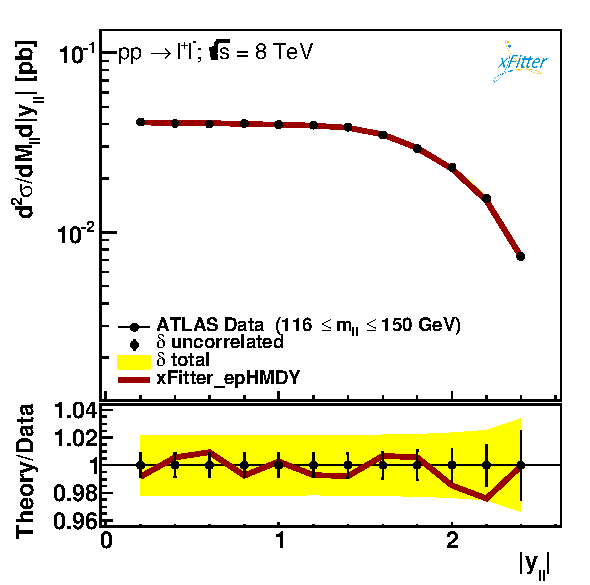
\includegraphics[width=7cm]{figs/data_401-1.pdf}
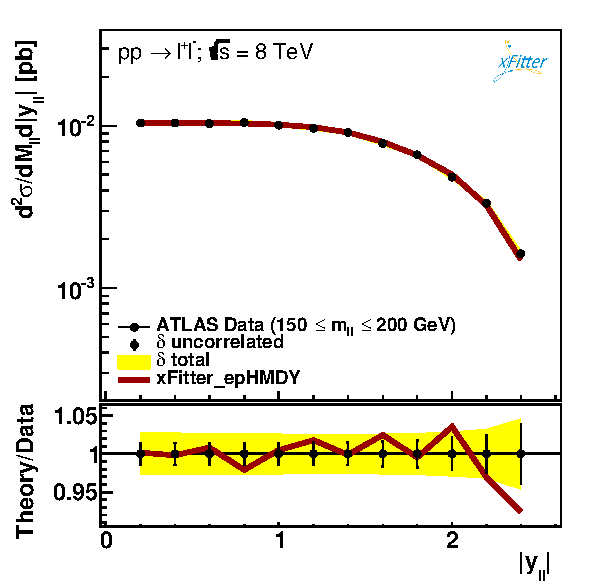
\includegraphics[width=7cm]{figs/data_402-1.pdf}
\caption{Comparison between the results of the fit and the ATLAS data
  for the $(m_{ll},|y_{ll}|)$ double-differential Drell-Yan cross-sections
  as function of $|y_{ll}|$, for the first two $m_{ll}$ bins.
  %
  The comparisons are shown both
  in an absolute scale (upper plots) and as ratios to the central value
  of the experimental data in each $y_{ll}$ bin (lower plots).
  %
  The error bars on the data points correspond to the bin-to-bin uncorrelated
  uncertainties, while the yellow bands
  indicate the size of the correlated uncertainties.
  %
  The solid lines indicate the theory calculations obtained using the results
  of the fit {\tt xFitter\_epHMDY}.
}
\label{hmDY_2D_1}
\end{figure}

%%%%%%%%%%%%%%%%%%%%%%%%%%%%%%
\begin{figure}[t]
\centering
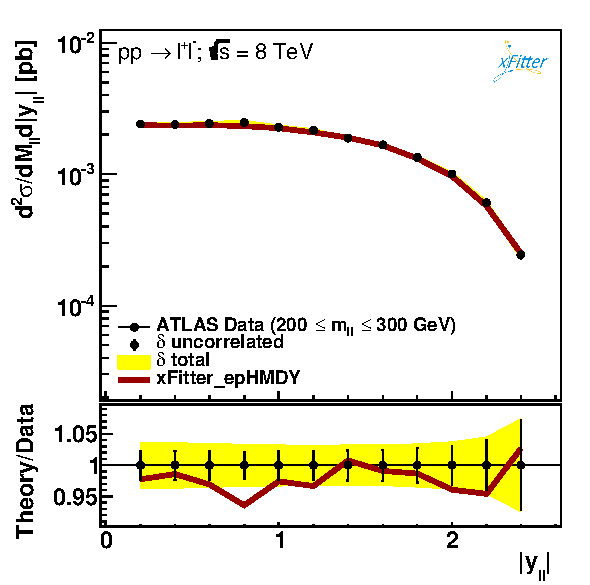
\includegraphics[width=7cm]{figs/data_403-1.pdf}
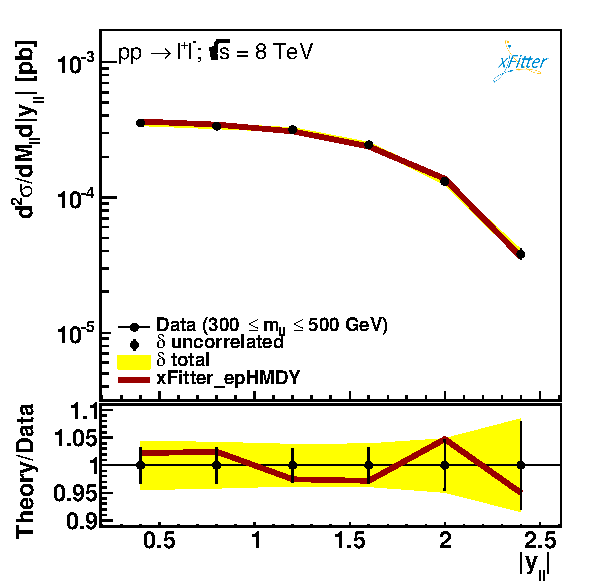
\includegraphics[width=7cm]{figs/data_404-1.pdf}
\caption{Same as Fig.~\ref{hmDY_2D_1} for the third and fourth $m_{ll}$ bins.
}
\label{hmDY_2D_2}
\end{figure}

%%%%%%%%%%%%%%%%%%%%%%%%%%%%%%
\begin{figure}[t]
\centering
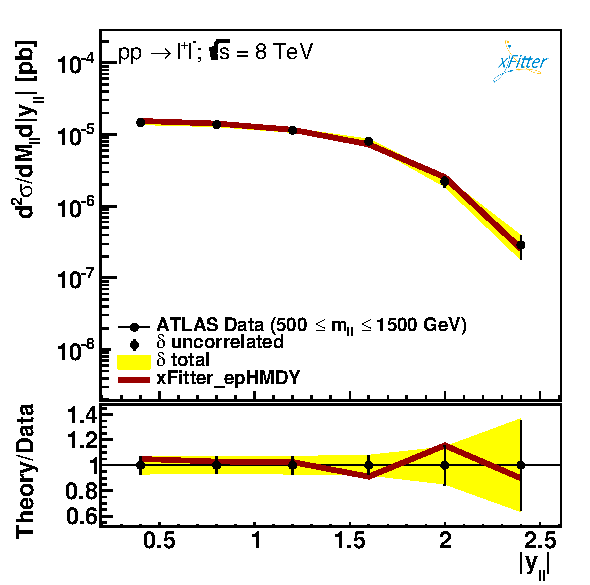
\includegraphics[width=7cm]{figs/data_405-1.pdf}
\caption{Same as Fig.~\ref{hmDY_2D_1} for the highest $m_{ll}$ bin.
}
\label{hmDY_2D_3}
\end{figure}
%%%%%%%%%%%%%%%%%%%%%%%%%%%%%%%

Figs.~\ref{hmDY_2D_1}--\ref{hmDY_2D_3} demonstrate
a good agreement between ATLAS data and the NNLO theory
predictions obtained from the {\tt xFitter\_epHMDY} fit.
%
This agreement is also quantitatively expressed by the values of the $\chi^2$ reported in
Table~\ref{tab:chi2fit}, where for the ATLAS data a $\chi^2/N_{\rm dat}=1$ is found.
%
This is particularly remarkable
given the high precision of the data, with total experimental
uncertainties at the few percent level in most of the kinematic range.

\subsection{The photon PDF from LHC high-mass DY data}

%We now present the results of the {\tt xFitter\_epHMDY}
%fit of the photon PDF $x\gamma$ and compare with
%other recent determinations. We will also assess the impact
%of the ATLAS high-mass DY data on the quark and gluon PDFs as compared
%to a fit with only HERA structure functions as input.

%%%%%%%%%%%%%%%%%%%%%%%%%%%%%%%%%%%%%%%%%%%%%%%%%%%%%%%%
\begin{figure}[t]
  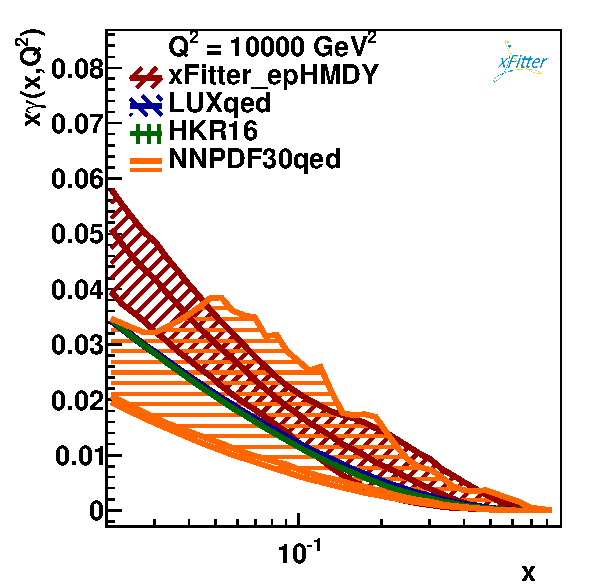
\includegraphics[width=7cm]{figs/photon_comp_10000.pdf}
  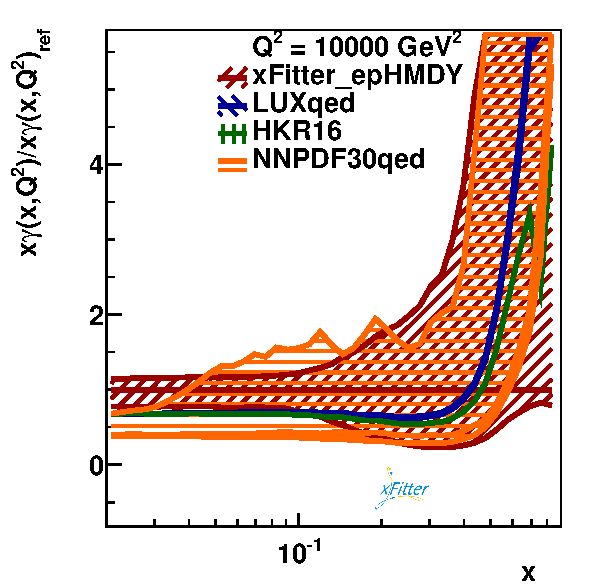
\includegraphics[width=7cm]{figs/photon_comp_10000_ratio.pdf} 
  \caption{Left plot: comparison between the photon $x\gamma(x,Q^2)$ at $Q^2=10^4$ GeV$^2$
    from the present NNLO analysis ({\tt xFitter\_epHMDY}) with the
    corresponding results from NNPDF3.0QED, LUXqed and HKR16.
  %
  Right plot: the same comparison, now with the results normalized to the central value
  of {\tt xFitter\_epHMDY}.
  %
  For the present fit, the PDF uncertainties are shown at the 68\% CL obtained from the MC method,
  while model and parametrisation uncertainties are discussed below.
  %
  For HKR16 only the central value is shown, while for LUXqed
  the associated PDF uncertainty band~\cite{Manohar:2016nzj} is included. }
\label{photon_zoom} \label{photon_zoom_ratio}
\end{figure}
%%%%%%%%%%%%%%%%%%%%%%%%%%%%%%%%%%%%%%%%%%%%%%%%%%%%%%%%

In Fig.~\ref{photon_zoom}, the photon PDF, $x\gamma(x,Q^2)$, is shown at
$Q^2=10^4$ GeV$^2$,  and it is compared to the corresponding LUXqed,
HKR16 and NNPDF3.0QED results.
%
In the left plot the comparison is presented in an absolute scale, while
in the right plot the ratio of
different results normalized to
the central value of the fit is shown.
%
For the present fit, {\tt xFitter\_epHMDY}, 
the experimental PDF uncertainties at the 68\% confidence level (CL) are obtained from the Monte Carlo method,
 while model and parametrisation uncertainties are discussed below.
 %
Likewise, the  NNPDF3.0QED PDF set is shown the 68\% CL uncertainty band,
while for LUXqed the associated PDF uncertainty band is computed according to the
prescription of Ref.~\cite{Manohar:2016nzj}.
 %
For HKR16, only the central value is available.
%
The $x$-range in Fig.~\ref{photon_zoom} has been restricted to the region
$0.02 \le x \le 0.9$, since beyond that region there is only limited sensitivity to $x\gamma(x,Q^2)$.

Fig.~\ref{photon_zoom} shows that for $x\ge 0.1$ the four determinations of
the photon PDF are consistent within PDF uncertainties.
%
For smaller values of $x$, the photon PDF from LUXqed and HKR16 is somewhat smaller than {\tt xFitter\_epHMDY},
but still in agreement at the 2-$\sigma$ level.
%
This agreement is further improved if the PDF uncertainties in
{\tt xFitter\_epHMDY}
arising from variations of the input parametrisation are added to experimental
uncertainties, as discussed in Sec.~\ref{sec:crosscheck}.
%
Moreover, the results of this work and NNPDF3.0QED agree at the 68\% CL for $x\ge 0.03$,
and the agreement extends to smaller values of $x$ once the parametrisation
uncertainties in {\tt xFitter\_epHMDY} are accounted for.
%
The LUXqed and the HKR16 calculations of $x\gamma(x,Q^2)$ are very close
to each other across the entire range of $x$.

Fig.~\ref{photon_zoom} shows that
for $0.04 \le x \le 0.2$ the present analysis  exhibits smaller PDF
uncertainties as compared to those from  NNPDF3.0QED.
%
Indeed, the experimental uncertainty on the {\tt xFitter\_epHMDY}
turns out to be at the  $\sim 30\%$ level for $x\le 0.1$.
At larger $x$ it increases rapidly
specially in the positive direction.
%
The reason for this behaviour at large $x$ can be understood by recalling that
variations of $x\gamma(x,Q^2)$ in the negative
direction are constrained by positiveness.
%
The limited sensitivity of the ATLAS data  does not allow a determination of $x\gamma(x,Q^2)$ with uncertainties
competitive with those of LUXqed, which are at the few percent level.

It is also interesting to assess the impact of the high-mass Drell-Yan 8 TeV measurements on
the light quark and gluon PDFs.
%
For this purpose, the fits have been repeated freezing the photon PDF to the
{\tt xFitter\_epHMDY} shape. 
%
This is necessary because
HERA inclusive data alone, which are the 
benchmark for this comparison, have no sensitivity to the photon
PDF.
%
This way, 
a meaningful comparison between the quark and gluon PDFs
from a HERA-only
baseline and the HERA+HMDY fit can be performed.
% with the effects of
%the photon PDF being factored out.

This comparison is shown in Fig.~\ref{fig:QCDfit} for the up and down
antiquarks $x\bar{u}(x,Q^2)$ and $x\bar{d}(x,Q^2)$, for which the effect of the high-mass Drell-Yan data is
expected to be most pronounced, since HERA inclusive cross sections
provide little information on quark flavour separation.
%
In Fig.~\ref{fig:QCDfit}, the $x\bar{u}(x,Q^2)$ and $x\bar{d}(x,Q^2)$ together
with the associated MC uncertainties have been computed
at the initial parametrisation scale of $Q^2=7.5$ GeV$^2$ and
are shown as ratios to the central value of the {\tt xFitter\_epHMDY}
fit.
%
The modifications in the medium
and large-$x$ antiquark distributions from the high mass DY data are
rather moderate.
%
%For $x\bar{d}$, the impact of the ATLAS DY data is negligible, while
%for $x\bar{u}$ it is somewhat larger, though still quite small,
%for $x\ge 0.05$.
%
It has been verified that the same conclusions can be derived
from fits obtained by switching
off the QED effects for both the HERA only fits and the HERA+HMDY fits.
%
Therefore, while the ATLAS high-mass Drell-Yan measurements have a significant constraint
on the photon PDF, their impact on the quark and gluon PDFs is moderate.

%%%%%%%%%%%%%%%%%%%%%%%%%%%%%%
\begin{figure}[t]
\centering
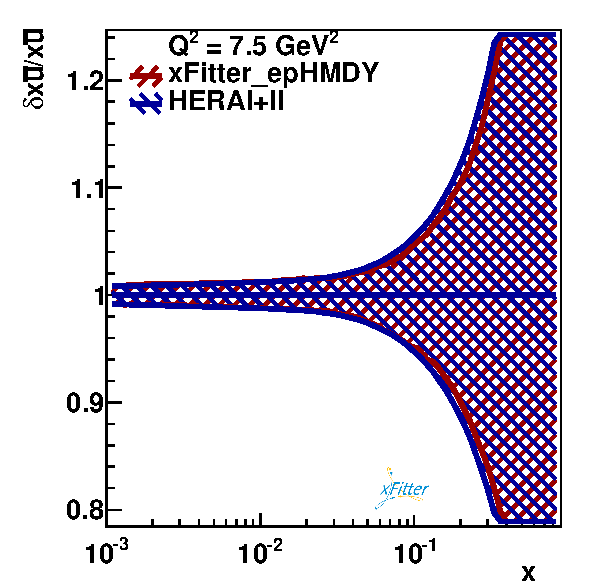
\includegraphics[width=7cm]{figs/q2_7_5_pdf_ubar_ratio.pdf}
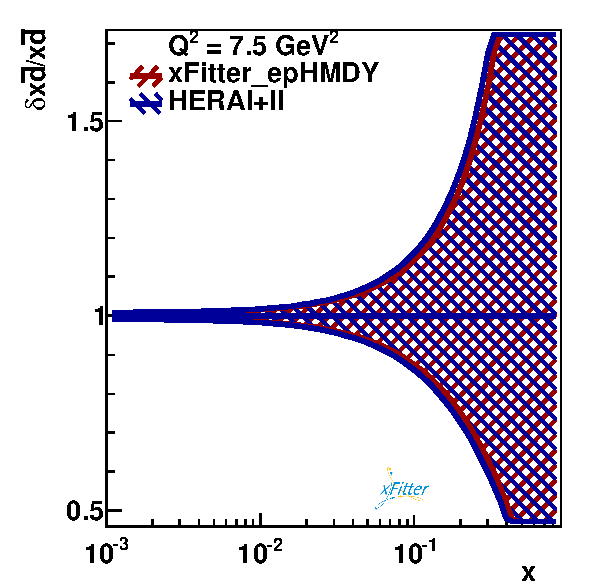
\includegraphics[width=7cm]{figs/q2_7_5_pdf_dbar_ratio.pdf} 
\caption{The impact of the ATLAS high-mass 8 TeV Drell-Yan measurements
  on the $x\bar{u}$ and $x\bar{d}$ sea quark PDFs at the input
  parametrisation scale $Q^2=7.5$ GeV$^2$.
  %
  The results are shown normalized to the central value of {\tt xFitter\_epHMDY}. 
  }
\label{fig:QCDfit}
\end{figure}
%%%%%%%%%%%%%%%%%%%%%%%%%%%%%%%

\subsection{Robustness and perturbative stability checks}
\label{sec:crosschecks}

Following the presentation of the main result of this work, the {\tt
  xFitter\_epHMDY} determination of the
photon PDF $x\gamma(x,Q^2)$, the robustness of this determination
with respect to a number of variations is assessed.
%
Firstly, variations in the values of the input
physical parameters, such as $\alpha_s$ or the charm mass are explored.
%
Secondly, variations of the choices made for the PDF input parametrisation
are considered.
%
Finally,
variations associated to different methodological choices in
the fitting procedure are quantified.
%
In each case, one variation at a time is performed 
and compared with the central value
of $x\gamma(x,Q^2)$ and its experimental PDF
uncertainties computed using the Monte Carlo method.

%%%%%%%%%%%%%%%%%%%%%%%%%%%%%%                                          
\begin{figure}[t]
\centering
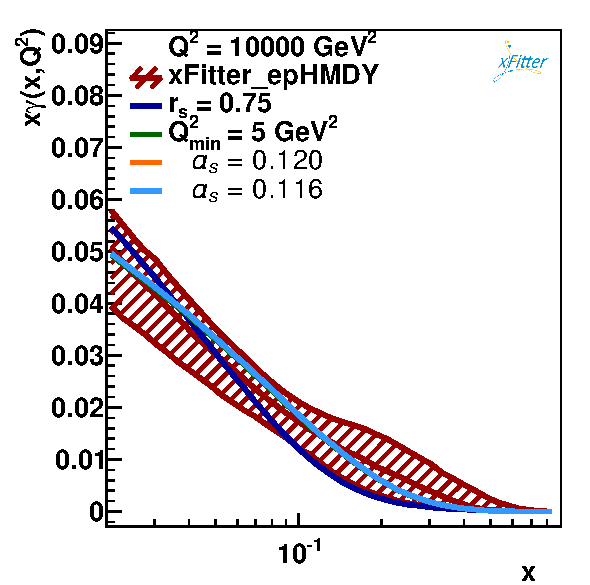
\includegraphics[width=7cm]{figs/q2_10000_pdf_ph_model_1}
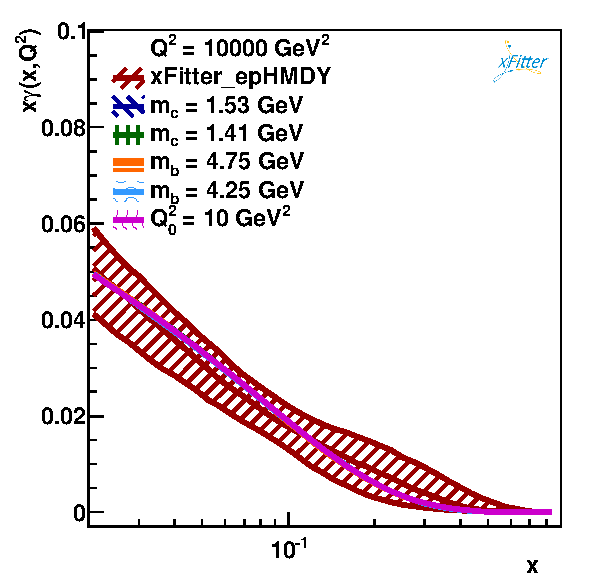
\includegraphics[width=7cm]{figs/q2_10000_pdf_ph_model_2}
\caption{Comparison between the baseline determination of
  $x\gamma(x,Q^2)$ at $Q^2=10^4$ GeV$^2$ in the present
  analysis, {\tt xFitter\_epHMDY},
  with the central value of a number of fits for which one input parameter has been varied.
  %
  The following variations have been considered: $r_s=0.75$, $Q^2_{\rm min}=5$ GeV$^2$, $\alpha_s=0.116$ and
  0.118 (left plot); and
  $m_c=1.41$ and 1.53 GeV, $m_b=4.25$ and 4.75 GeV, and $Q_0^2=10$ GeV$^2$ (right plot).
  %
  See text for more details about these variations.
}
\label{fig:model}
\end{figure}
%%%%%%%%%%%%%%%%%%%%%%%%%%%%%%

First the impact of uncertainties associated to either
the choice of input physical parameters or of specific settings
adopted in the fit is considered.
%
Fig.~\ref{fig:model} shows the comparison between the
{\tt xFitter\_epHMDY} 
determination of $x\gamma(x,Q^2)$ at $Q^2=10^4$ GeV$^2$, including the experimental MC
uncertainties, with the central
value of those fits for which a number of variations have been
performed.
%
Specificaly:
\begin{itemize}
\item The strong coupling constant is varied by $\delta \alpha_s=\pm 0.002$ around the central value.
\item The ratio of strange to non-strange light quark PDFs is decreased to $r_s=0.75$ instead of $r_s=1$.
\item The value of the charm mass is varied between $m_c=1.41$ GeV and $m_c=1.53$ GeV,
  and that of the bottom mass between $m_b=4.25$ GeV and $m_b=4.75$ GeV.
\item The minimum value $Q_{\rm min}^2$ of the fitted data is decreased down to $5$ GeV$^2$.
\item The input parametrisation scale $Q_0^2$ is raised to $10$ GeV$^2$ as compared
  to the baseline value of $Q_0^2=7.5~$GeV$^2$.
\end{itemize}
The results of Fig.~\ref{fig:model} highlight that in all cases effect
of the variations considered here is contained within (and typically much smaller than) 
the experimental PDF uncertainty bands of the reference fit.
%
The largest variation comes from the strangeness ratio $r_s$, where the resulting
central value turns out to be at the bottom end of the PDF uncertainty band for $x\ge 0.1$.

Another important check of the robustness of the present determination of
$x\gamma(x, Q^2)$ can be obtained by comparing the baseline fit with further
fits where a number of new free parameters are allowed in the PDF
parametrisation, in addition to those listed in Eq.~(\ref{eq:param}).
%
Fig.~\ref{fig:param} shows the impact of three representative
variations (others have been explored, leading to smaller
differences): more flexibility to the gluon distribution, allowing it
to become negative at the initial scale (labeled by ``${\rm neg}$''), in addition to $D_{u_v}$,
and then $D_{\bar{u}}+D_{\bar{d}}$.
%
As before, all variations are contained within the experimental PDF uncertainty
bands, though the impact of the parametrisation variations is typically larger
than that of the model variations: in the case of the
${\rm neg}+D_{\bar{u}}+D_{\bar{d}}$ variations, the central value is
at the lower edge of the PDF uncertainty band in the entire range
of $x$ shown.
%
%Importantly, once this additional source of PDF uncertainty arising from the
%parametrisation variations is accounted for, the agreement of the {\tt xFitter\_epHMDY}
%fit 
%with the LUXqed and HKR16  determinations
%shown in Fig.~\ref{photon_zoom} improves in the
%region around $x\simeq 0.02$.

A cross-check of the robustness of the estimated
experimental uncertainty of the photon PDF in this analysis is provided by the
comparison of the Monte Carlo and Hessian methods.
%
Fig.~\ref{fig:photon_mc_vs_hessian} shows this comparison
indicating a reasonable agreement between the two methods.
%
In particular, the central values of the photon obtained with the two
fitting techniques are quite similar to each other.
%
As expected, the MC uncertainties tend to be larger than the Hessian ones,
specially in the region $x\gsim 0.2$, indicating deviations with respect
to the Gaussian behaviour of the photon PDF.

%%%%%%%%%%%%%%%%%%%%%%%%%%%%%%%%%%%
\begin{figure}[t]
\centering
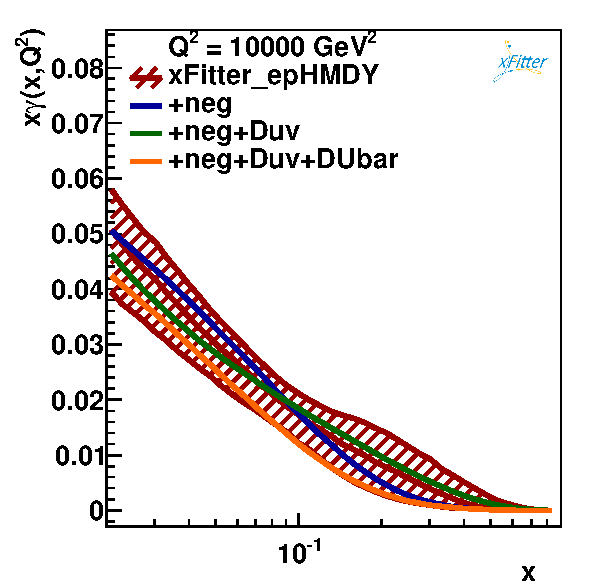
\includegraphics[width=7cm]{figs/q2_10000_pdf_ph_param_var.pdf}
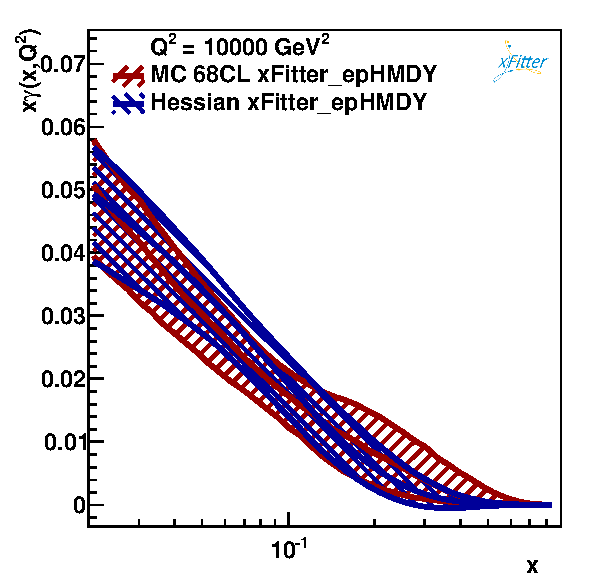
\includegraphics[width=7cm]{figs/photon_mc_vs_hessian} 
\caption{Left: the impact on the photon PDF $x\gamma(x,Q^2)$
  from {\tt xFitter\_epHMDY}
  in fits where a number of additional free parameters are allowed
  in the PDF parametrisation Eq.~(\ref{eq:param}).
  %
  The parametrisation variations that have been explored
  are: more flexibility to the gluon distribution, allowing
  it to become negative
  (labeled by ``${\rm neg}$''), adding on top $D_{u_v}$, and then
  adding $D_{\bar{u}}+D_{\bar{d}}$.
 %
 Right: comparison between the {\tt xFitter\_epHMDY} determinations obtained with the
 Monte Carlo (baseline) and with the Hessian methods, where in
  both cases the PDF error band  shown corresponds to the 68\% CL uncertainties.  }
\label{fig:param}
\label{fig:photon_mc_vs_hessian}
\end{figure}
%%%%%%%%%%%%%%%%%%%%%%%%%%

To complete these studies, an interesting exercise is to quantify the perturbative stability of
the {\tt xFitter\_epHMDY}
determination of the photon PDF $x\gamma(x,Q^2)$ with respect to the inclusion
of NNLO QCD corrections in the analysis.
%
To study this, Fig.~\ref{fig:nlo_vs_nnlo} shows a
comparison between the baseline fit of $x\gamma(x,Q^2)$, based on NNLO
QCD and NLO QED theoretical calculations, with the central value resulting from a
corresponding fit
based instead on NLO QCD and QED theory.
%
In other words, the QED part of the calculations is identical in both cases.
%
For the NNLO fit, only the experimental PDF uncertainties, estimated
using the Monte Carlo method, are shown.
%
From the comparison of Fig.~\ref{fig:nlo_vs_nnlo}, it is clear that the
fit of $x\gamma(x,Q^2)$ exhibits a reasonable perturbative stability,
since the central value of the NLO fit is always contained in the
one-sigma PDF uncertainty band of the baseline {\tt xFitter\_epHMDY} fit.
%
The agreement between the two fits is particularly good for
$x\gsim 0.1$, where the two central values are very close to each
other.
%
This comparsion is shown at low scale, $Q^2=7.5$ GeV$^2$ and high scales $Q^2=10^4$ GeV$^2$,
indicatring that perturbative stability is not scale dependent.

%%%%%%%%%%%%%%%%%%%%%%%%%%%%%%%%%%%%%%%%%%%%%%%%%%%%%%%%%%%%%%%%%%%%%%%%%%%%%%%%%%%%%%%%%%%%%
%%%%%%%%%%%%%%%%%%%%%%%%%%%%%%%%%%%%%%%%%%%%%%%%%%%%%%%%%%%%%%%%%%%%%%%%%%%%%%%%%%%%%%%%%%%%%
\begin{figure}[t]
\centering
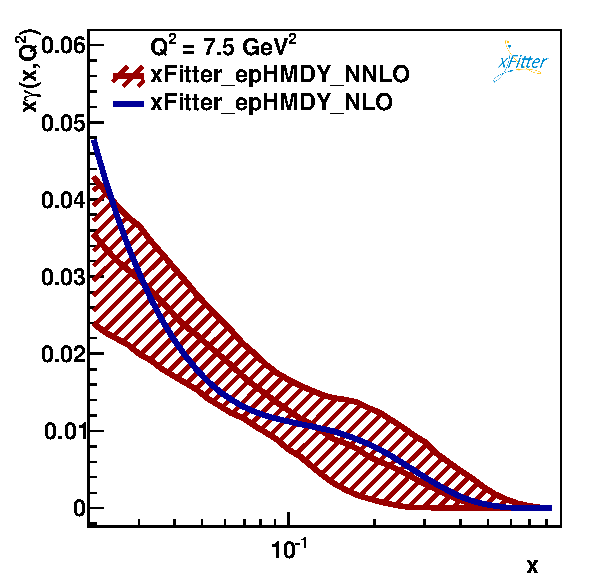
\includegraphics[width=7cm]{figs/q2_7_5_pdf_ph_NLOvsNNLO.pdf}
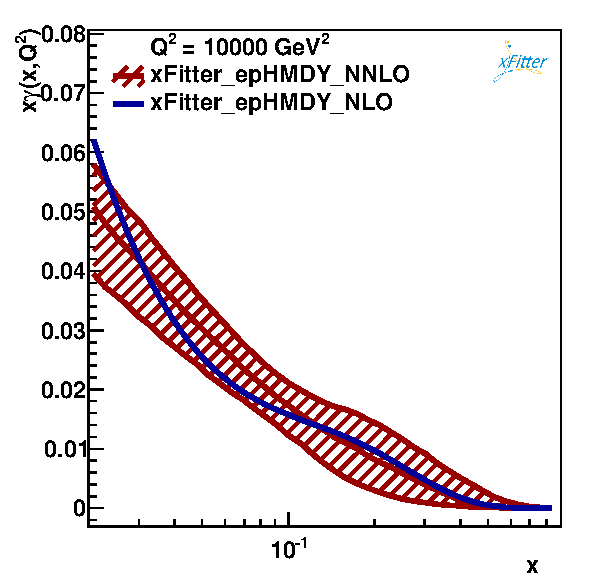
\includegraphics[width=7cm]{figs/q2_10000_pdf_ph_NLOvsNNLO.pdf}
\caption{Left plot: comparison between the reference {\tt xFitter\_epHMDY}
  fit of $x\gamma(x,Q^2)$, based on  NNLO QCD and NLO QED theoretical
  calculations, with the central value of the corresponding fit based
  on NLO QCD and QED theory, at $Q^2=7.5$ GeV$^2$.
  %
  In the former case, only the experimental Monte Carlo PDF
  uncertainties are shown.
  %
  Right plot: same comparison, now presented at the higher scale of $Q^2=10^4$ GeV$^2$.  }
\label{fig:nlo_vs_nnlo}
\end{figure}
%%%%%%%%%%%%%%%%%%%%%%%%%%%%%%%%%%%%%%%%%%%%%%%%%%%%%%%%%%%%%%%%%%%%%%%%%%%%%%%%%%%%%%%%%%%%
%%%%%%%%%%%%%%%%%%%%%%%%%%%%%%%%%%%%%%%%%%%%%%%%%%%%%%%%%%%%%%%%%%%%%%%%%%%%%%%%%%%%%%%%%%%%
